\chapter{Supervised Learning}\label{ch_supervised}
\chapterauthor{Jeff Yoshimi}

% Need more on generalization
% Mention self-supervised learning somewhere and link to transformer chapter

With \glossary{supervised learning}, parameters (weights and biases) are updated using an explicit representation of how we want the network to behave. Input vectors in an \glossary{input dataset} are associated with targets or labels in \glossary{target dataset} (see section \extref{datasets}).\footnote{More review from chapter \extref{ch_data_science}: recall that the input and target dataset together are a \glossary{labeled dataset} and that the part of the data we use to train a network is the \glossary{training subset} of the data. Also recall that the term `label' is sometimes reserved just for classification tasks but is also (as here) sometimes used to refer to target data for regression tasks as well.}  We say, ``if you see this pattern, produce this other pattern.'' This is sometimes called ``learning with a teacher.'' We saw in chapter \extref{ch_unsupervised} that Hebbian pattern associators can be trained by exposure to input / output pairs. Unfortunately, that method is unstable. The weights tend to explode to extreme values. So we need something more adaptive and robust: a way to get the weights to go up and down and settle in on just the right values, so that our network gets as close as possible to doing what we want. It's a bit like Goldilocks, trying to find the breakfast whose temperature is not too hot, not too cold, but just right.\footnote{This is sometimes called the `Goldilocks principle'. See \url{https://en.wikipedia.org/wiki/Goldilocks_principle}.} Supervised learning algorithms provide a way to achieve this kind of zeroing in on just the right solution to a problem.

In this chapter we focus on general features of supervised learning in feed-forward networks, developing a toolkit of  techniques and visualization methods. We will need to think clearly about labelled datasets, distinguish classification from regression tasks, learn how to visualize these two kinds of task, and discuss how to compute a metric of how well our network is doing at a given time (``error''). Finally, we will need to think about error \emph{reduction} in a visual way, as downward motion on an error surface using the method of ``gradient descent'', which is basically the dynamical systems idea from chapter \extref{ch_dst} of finding attracting fixed points, but this time in weight space rather than activation space. 
% Make a bit more of the fixed point link

In chapter \extref{ch_lms_backprop}, we cover some of the main classes of algorithm in supervised learning for feed-forward networks (including deep networks), and discuss their implications for cognitive science. In chapter \extref{ch_supervised_recurrent}, we discuss how supervised learning methods can be used to train recurrent networks, and how these trained recurrent networks have illustrated ideas in cognitive science. In both cases, we will see that internal representations are often learned by these networks, which seem to be similar to those humans use in processing language, recognizing faces, and in other tasks. 

% Use function approximation language from Deep Learning?
% Wiki ``Supervised learning is the machine learning task of inferring a function from labeled training data''

\section{Labeled datasets}\label{supervised_datasets}

With supervised learning, we tell the network what we want it to do. There is a teacher or trainer. Recall from chapter \extref{ch_data_science} that a \glossary{labeled dataset} for a supervised learning task consists of a pair of datasets: an input dataset and a target dataset. Both datasets contain the same number of rows.
% Mention y_r as well.
% Integrate: Since the rows of the tables are vectors (see chapter \extref{ch_linear_algebra}) they are represented here by bold faced symbols, like $\mathbf{t}_r$ and $\mathbf{y}_r $. 

We will say that a labeled dataset is \emph{compatible} with a feed-forward neural network if (1) the number of columns in the input dataset is the same as the number of input nodes in the network, and (2) the number of columns in the target dataset is the same as the number of output nodes in the network. The network can have any number of hidden layers and still be compatible with the dataset. A labeled dataset can be used to train any network compatible with it. Examples of labeled datasets and compatible networks are shown in figure \ref{tables_nets}. 

A labeled dataset can be thought of as a contract for a pattern association task: we'd like to train a network to come as close possible to implementing the input-output associations described by our labeled dataset. In the language of vector-valued functions, we are training a network to approximate a function that associates each vector in the input dataset with the corresponding target vector in the labeled dataset.

\begin{figure}[h]
\centering
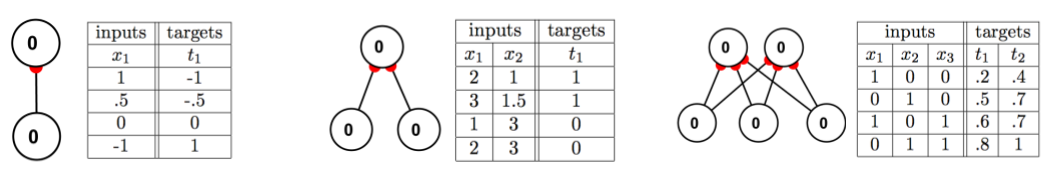
\includegraphics[scale=.4]{./images/TablesAndNets.png}
\caption[Jeff Yoshimi.]{Some labeled datasets and the types of neural network topologies those training sets could be used on. Each dataset contains an input dataset and a target dataset with 4 rows. In each case, the input dataset has as many columns as its paired network has input nodes and the target dataset has as many columns as its paired network has output nodes. A classification task is shown in the middle (binary valued targets) and regression tasks are shown on the left and right (real-valued targets).}
\label{tables_nets}
\end{figure}

\section{Supervised Learning: A First Intuitive Pass}\label{SupervisedFirstPass}

In this chapter we focus on feed-forward networks, which can be thought of implementing vector valued functions (such networks are often referred to as ``MLP's'' or ``Multi-Layer Perceptrons'', in reference to earlier work by Widrow and others; see chapter \extref{ch_history}). A labeled dataset is essentially a specification for a vector-valued function we'd like our compatible network to implement. Given an input vector $\mathbf{x}_r$ in a labeled dataset, we want the network to produce an output vector $\mathbf{y}_r$ as close as possible to the the corresponding target vector in that dataset. 
%Given an input vector $\mathbf{x}_r$ in the input dataset, we want the network to produce an output vector $\mathbf{y}_r = N(\mathbf{x}_r)$ in the target dataset. 

% A labeled dataset compatible with $N$, containing an input dataset and a target dataset. The rows of the input dataset are $\mathbf{i}_i$, the the rows of the target dataset are $\mathbf{t}_i$, and the outputs of $N$ (the output dataset) are $\mathbf{y}_i$. Note that if we refer to $\mathbf{i}_i$ and $\mathbf{t}_i$, for example, we are referring to the  "corresponding" rows of the two datasets.

The way we do this with supervised learning is by using algorithms that modify the \glossary{parameter}s  $p_1,\dots,p_n$ of the network (the parameters are usually taken to be the weight strengths and the biases on all nodes except the input nodes). We start out with a network all of whose parameters $p_i$ have been initialized to random values.\footnote{When I refer to``randomizing'' a set of values, we mean setting them to values generated by a probability distribution, \eg a uniform or a Gaussian distribution.}  It's like making a network in Simbrain and pressing the \texttt{w} then \texttt{r} buttons, which selects all the weights and randomizes them. Recall from Chap. \extref{ch_dst} that parameters are variables associated with a dynamical system that are fixed when the system is run but can be changed between runs. In a recurrent network, parameters determine the network's dynamics. In a feed-forward network, they determine the vector-valued function it approximates. Our goal is to set the parameters of the network so that it implements a vector-valued function that reproduces the associations in the labeled dataset as closely as possible.
%so that $N(\mathbf{x}_r) \approx \mathbf{t}_r$ for each row $r$ of the labeled dataset.
% \footnote{When neural networks are not being trained, weights are thus parameters in the dynamical systems sense. However, when training begins, the parameters become state variables of a new dynamical system on the weight space of the network (more on this in section \ref{sect_gradient_descent}).} 
% The two topics come together with supervised recurrent, where we train parameters to produce a _desired_ dynamics, roughly speaking
 
Because we start with random values for the parameters of the network, it will generally not do well at first. Its outputs won't  initially match target values. We then use a learning algorithm (several are covered in chapter \extref{ch_lms_backprop}) to incrementally update the parameters. If all goes well, the network should begin to behave in accordance with the specifications of the labeled dataset.

Below we refer to ``errors''  and ``overall error'', which are discussed in greater detail in Sect. \ref{sect_error}. Roughly speaking individual errors says how far away the outputs produced by a network relative to an input are from the target values for that input, and overall error combines these errors together into a single number for all the nodes and all the rows of the dataset.
% Overall error could be batch error. See pytorch conventions and the convention of "reducing" the error using sum or mean.  Give "individual error" a better name, like error for one training example. We used to use row error, which I like, and maybe we can bring it back. See the footnote below around line 186

To train a network, we select a subset of a compatible labeled dataset, a \glossary{training subset} (section \extref{generalization}). This is our ``training data'': a set of input vectors and target vectors in a subset of a labeled dataset that we use to train our model. A schematic of the process that applies to most forms of supervised learning is as follows:
 \begin{enumerate}
\item Randomize network's parameters $p_1,\dots,p_n$.
\item For each row $\mathbf{x}_r$  of the input dataset:
\begin{enumerate}
\item Set the input-layer activations of the network to $\mathbf{x}_r$.
\item Compute the network's output vector $\mathbf{y}_r$. 
\item Compute output errors by comparing the targets $\mathbf{t}_r$ with the outputs $\mathbf{y}_r$ (for each output, subtract the output from the target).
\item Update $p_1,\dots, p_n$ with the goal of reducing errors (so that outputs are closer to targets).
\end{enumerate}
\item Repeat step 2 until overall error is sufficiently low.
\end{enumerate}
	
% Mention stochastic gradient descent and mini-batch as variations on this. 
% Introduce the term epoch to refer to one pass through the entire dataset. Bold face these some of these terms for the glossary.
% Discuss testing dataset, and return to the discussion of generalization. This also matches the tensorflow demo.

We will see that this can be visualized in geometric way, as ``gradient descent'' to a low point on an ``error hypersurface.''


\section{Classification and Regression}\label{classificationRegression}

% https://commons.wikimedia.org/wiki/File:Perceptron_example.svg
% Useful text on regression vs. classification: Bishop p. 194. 
For feed-forward networks trained using supervised learning, an important distinction can be made between classification and regression tasks. At a first pass, classification tasks associate inputs with categories, and regression tasks associate inputs with numbers.\footnote{These concepts (especially classification) can also be applied to unsupervised learning. Recall from chapter \extref{ch_unsupervised} the discussion of competitive networks and self organizing maps, which learn to classify inputs into distinct categories without a teacher. The distinction also applies to recurrent networks, which can learn to classify  dynamic inputs, for example, or to produce dynamic real valued outputs.} 

In a \glossary{classification task}, the network sorts inputs into categories. The inputs might be the height and weight of a person, and the output will be a prediction about whether that person is a child or adult. Or, the network could take car data as input, and predict whether the car is a sports car or economy car. Notice that in both cases the outputs are categorical: they say which of $n$ categories something falls in. This is one-of-$k$ or one-hot encoding, discussed in chapter \extref{ch_data_science}. One node for each category, and the one that's on corresponds to the category being classified. The three object detector (figure \extref{3ObjectClassifier}) is a classifier, which classifies smell inputs into one of three categories: Fish, Gouda, and Swiss. Figure \ref{F:letter_classify} shows an example of a feed-forward network that classifies pixel patterns as one of 26 letters.
% Note threshold activation function historically, and softmax for cases where outputs are probabilities

\begin{figure}[h]
\centering
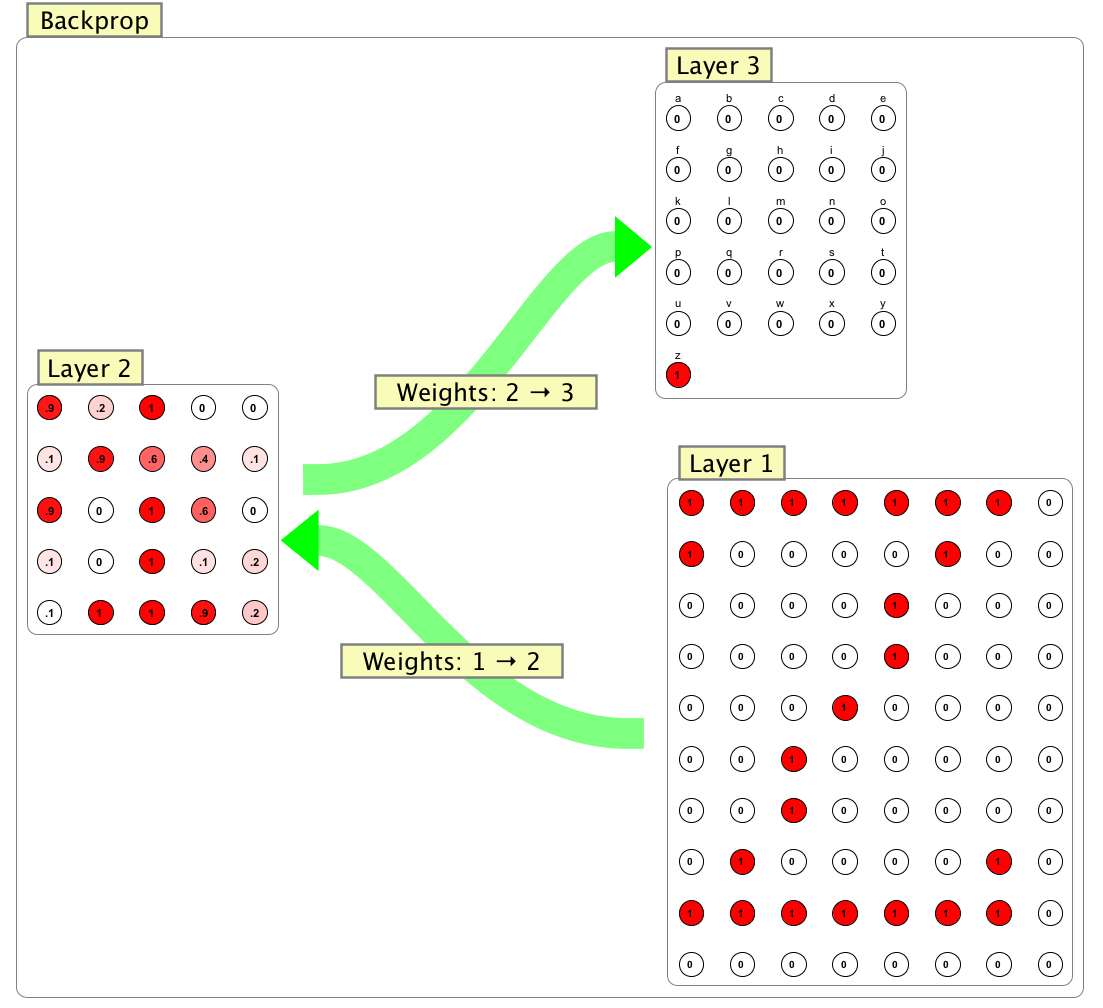
\includegraphics[scale=.4]{./images/letterClassification.png}
\caption[Simbrain screenshot.]{An example of classification. A feed-forward network trained via supervised learning to classify letter inputs as specific letters.}
\label{F:letter_classify}
\end{figure}

In a \glossary{regression task}, a network trained has real valued target values. This is simply the more general case of estimating a vector-valued function, where there are no constraints on how we interpret the outputs. If we train a network to predict the speed of a car (quarter-mile time) based on its fuel efficiency, engine size, and how many cylinders it has, we have a regression problem. We are not classifying cars into types, but predicting a numerical quantity about cars: their speed in a drag race.

% (See Duda-Stork 1-d examples)
% Emphasize that regression is closer to the concept of function approximation . Classification is a different conceptual game, and a bit easier to start with. Could use this as the running thread.

% Improve. Blue dots. Perhaps make 2 node network vertical.
\begin{figure}[h]
\centering
\raisebox{-0.5\height}{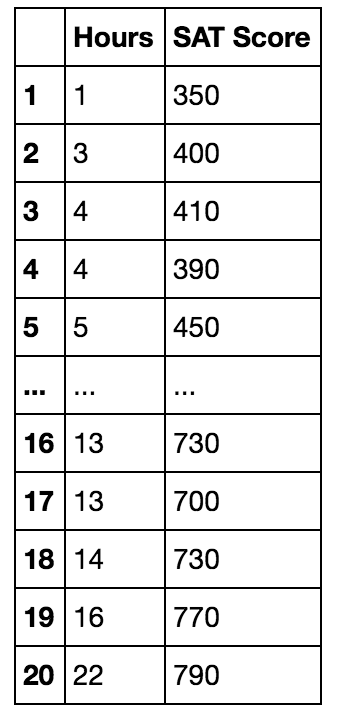
\includegraphics[scale=.35]{./images/linearRegressionTable.png}}
\hspace*{.4in}
\raisebox{-0.5\height}{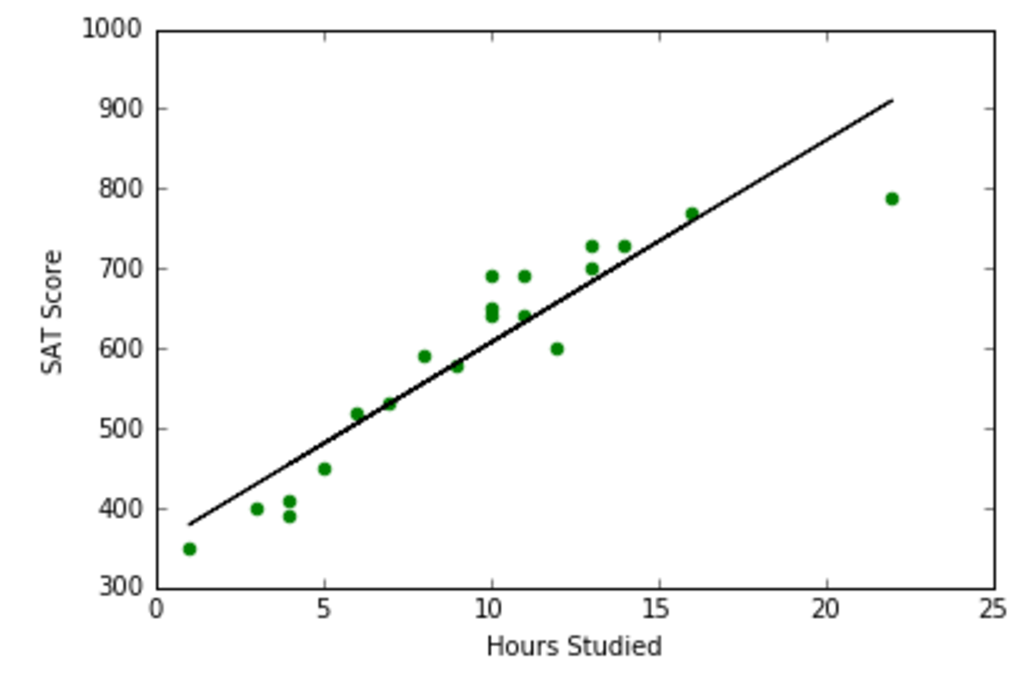
\includegraphics[scale=.4]{./images/linearRegression.png}}
\hspace*{.4in}
\raisebox{-0.5\height}{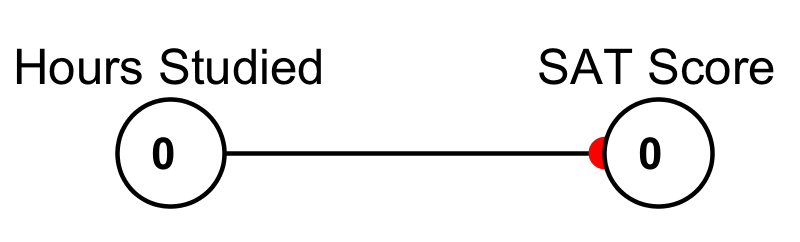
\includegraphics[scale=.3]{./images/2Node_Network.png}}
\caption[Jeff Yoshimi.]{An example of regression. (Left) The data used to train the network. Hours of study vs. score on the SAT. (Middle) A plot of the data with a regression line. These are points in an input-target space, as discussed in chapter \extref{ch_supervised}. This line can be used to predict how well someone will do based on how much they study. (Right) A simple 2-node network that could implement this regression solution. Enter hours studied in the input node, and it should display a  predicted SAT score in the output node.}
\label{F:linearRegression}
\end{figure}
% Todo: Where did this data come from? 

The term ``regression'' comes from the statistical technique of linear regression. In fact, neural networks provide a nice way to understand what linear regression is. To understand this, consider a classic example of linear regression: predicting how well someone will do on a test based on how many hours they study. As can be seen in figure \ref{F:linearRegression}, the more you study, the higher your score is likely to be. We can fit a line to this data using standard statistical techniques. But a neural network--like the one shown in the right panel of the figure--can also do it.\footnote{Note that in this example, the data have not been rescaled (chapter \extref{ch_data_science}). Rescaling is often important, but not always necessary.} That network can be trained to predict SAT scores based on hours studied. Look how simple it is!  That's all linear regression really does: it gives us a network that we can use to make predictions, in this case, simple predictions where a single input produces a single output. In fact, the details are also pretty straightforward. In this case, the slope of the line corresponds to the weight, and the intercept is the bias on the linear output node. Recall $y=mx + b$ from high school math class; here $y$ is the output activation, $x$ is the input activation, $m$ is the weight, and $b$ is the output node bias. Thus, in computing weighted inputs for the output node, when there is just one input, we are just computing a simple linear function.

Of course we can get more complex. We can have multiple inputs. We can  predict how tall a tree will be based on its age, average rainfall where it is planted, and concentrations of chemicals in its soil. In that case we have multiple inputs predicting one output. In statistics this is called \emph{multiple regression}, but you can see that it's just a matter of having  a many-to-one network where we estimate the values of the weights and biases. When we have multiple outputs we just repeatedly use this technique on each output node. One output node predicts the height of the tree, another predicts how long it will live, etc. That is called \emph{multi-variate multiple regression}. Thus networks with many inputs and many outputs can  be understood as performing regression tasks.

As a simple procedure for deciding whether a task is a classification or regression task, look at the target data. If the target data represent categories, e.g. a one-hot encoding, it is probably a classification task. If they are real-valued or otherwise numerical data, then it is probably a regression task. Even more simply: classification tasks typically involve binary or discrete valued targets, while regression tasks typically involve real-valued targets. 

\section{Visualizing Classification as Partitioning an Input Region into Decision Regions}
\label{visClassification}

% In all classification plots plot classes of two points in a different color. Then it coheres with the python example better.
% Could show how the pictures are related. Show a function surface and then a threshold and their intersection is the decision surface. Something like that.

% An outstanding source on these issues: http://colah.github.io/posts/2014-03-NN-Manifolds-Topology/

It is important in supervised learning to be able to conceptualize problems in terms of a set of graphical ideas. They are familiar ideas, and not too hard, but they confusingly overlap, so we must be careful and systematic about understanding them. You will see many diagrams that look quite similar. We will only be able to visualize what's going on directly for very small networks, but we can use these ideas to generalize to higher dimensions, which will give us a conceptual template for understanding more complex cases. This theme of visualizing ideas directly in small networks and then extending them to higher dimensions is often useful, as we will see.

The goal of a classification task is to create a model that correctly classifies inputs into a finite set of categories. Target values are binary; an input is either in a given category or not. Classification involves creating decision boundaries between inputs for the different categories. In this section we focus on decision regions produced by networks with a single weight layer and a single output node with a threshold activation function, but the ideas generalize in interesting ways to more complex networks (see Bishop \cite{bishop1995neural}, chapter 3).
% Threshold vs. linear or sigmoidal activation functions

% Fix all the graphics. Datapoints in blue, models in black. Next two figures.
\begin{figure}[h]
\centering
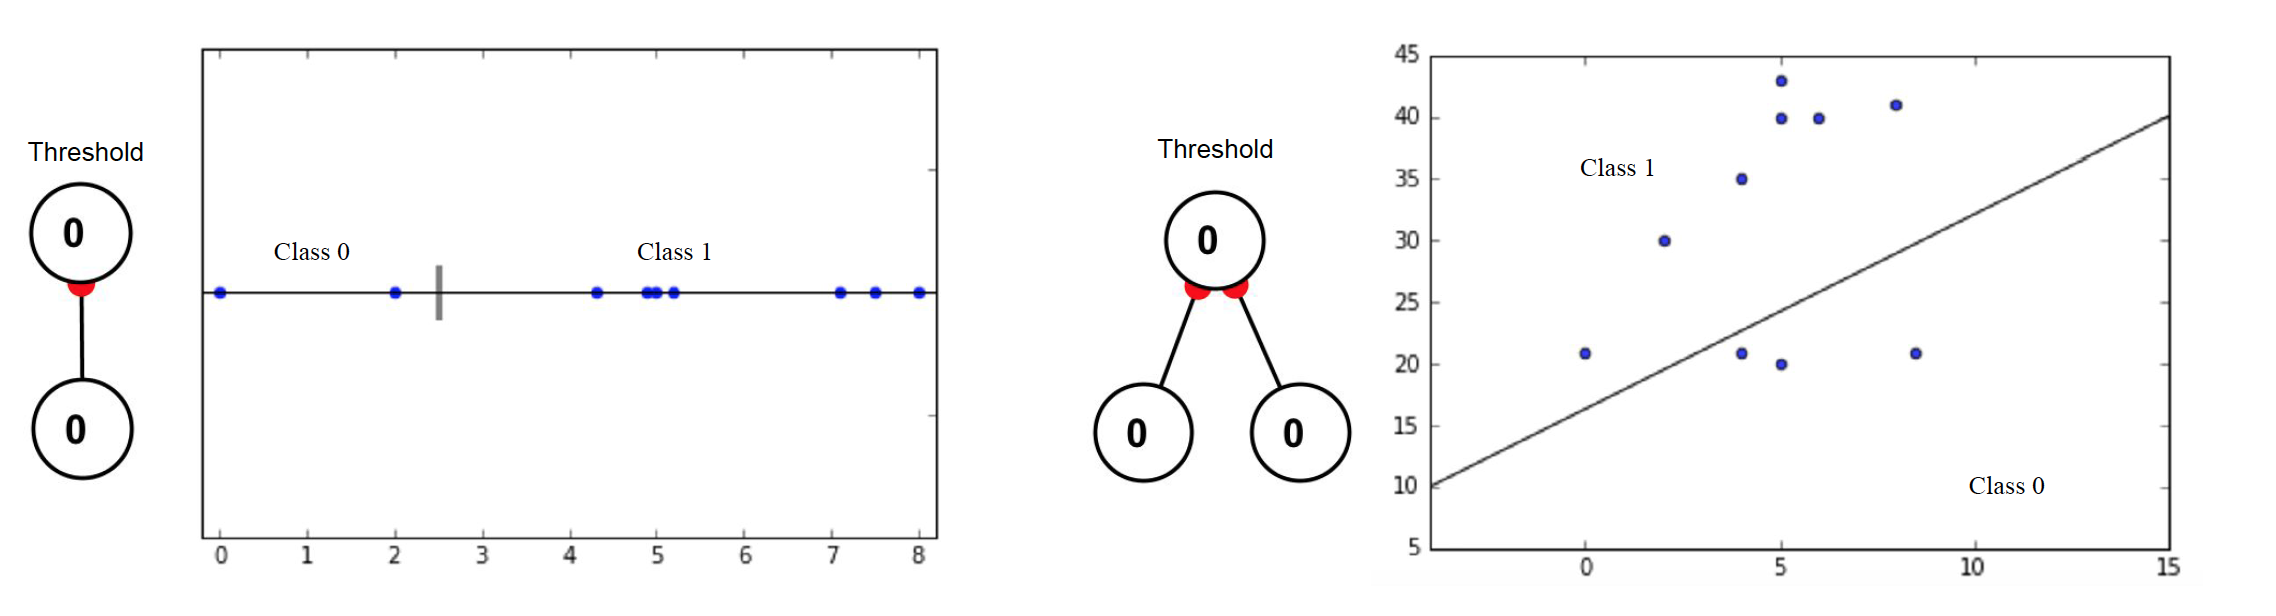
\includegraphics[width=0.9\textwidth]{images/visualizeClassification.png}
\caption[Jeff Yoshimi.]{A classification task for a 1-1 network (Left) and a 2-1 network (Right). Both networks use threshold activation functions on the output nodes. Points in the input space are shown in  blue. The decision boundaries between points classified as 0 or 1 are shown in gray. On the left, the decision boundary is a point shown as a small vertical hatchmark. On the right, the decision boundary is a diagonal line. The decision boundaries partition the input spaces into two decision regions, corresponding to outputs of 0 or 1.}
\label{visualize_classification}
\end{figure}

Simple linear networks using threshold activation functions partition the input space into \glossary{decision regions} separated by lines, planes, and hyperplanes (a hyperplane is intuitively a plane in an high dimensional space). Figure \ref{visualize_classification} shows classification tasks for 1-1 and 2-1 networks. In each case, the output node has a threshold activation function and the network is being trained to classify inputs into one of two classes. When the output node turns on (weighted inputs above threshold), the input is in class 1. When the output node is off, the input is in class 0. On the left, the input space is 1-dimensional, since there is one input node. The threshold functions divide the 1-dimensional input space into decision regions  labeled ``class 0'' and ``class 1'', via a \glossary{decision boundary}, in this case a 0-d point (represented by a hatchmark in the graph). On the right, the input space is 2-dimensional, and the decision boundary is 1-dimensional. The line again partitions the input space into two decision regions, for ``class 0'' and ``class 1.'

These ideas generalize to higher dimensions. The \emph{input space} will in general have as many dimensions as there are input nodes. The small networks in Figs. \ref{visualize_classification} and \ref{visualize_regression}  have 1 and 2-d input spaces. A network with 5000 input nodes has a 5000-dimensional input space. The \emph{decision boundary} in the input space of a network has as many dimensions as the number of input nodes minus 1. In the 5000-input node case, with one output node, the decision boundary is a 4999-dimensional hyperplane that divides the input space into two decision regions.

To summarize, for classification tasks we have:
\begin{description}
\item[Input space:] the vector space corresponding to the input nodes of a network. It has as many dimensions as there are input nodes. In the cases shown in figure \ref{visualize_classification} the input spaces are 1 and 2 dimensional.
\item[Decision boundary:] a point, line, or surface separating the input space into decision regions corresponding to distinct categories. The boundary has as many dimensions as the number of input nodes minus one. In the cases shown in figure \ref{visualize_classification} the decision boundaries are $1-1=0$ dimensional (a point) and $2-1=1$-dimensional (a line). 
\end{description}
% Went from linear case with hyperplanes to general case with hypersurfaces. Better manage transition, or talk more about general case of other functions, many linear nodes (many lines), wta (voroni cells), multi-layer, etc.
		
\section{Visualizing Regression as Fitting a Surface to a Cloud of Points}
\label{visRegression}

The goal of a regression task is to create a network that produces outputs as close as possible to a set of datapoints. Targets are real-valued. We can conceptualize regression as fitting a hypersurface (a generalization of lines, planes, and other surfaces to arbitrary dimensions)\footnote{See \url{https://en.wikipedia.org/wiki/Hyperplane}. An even more general concept is a hypersurface: \url{https://en.wikipedia.org/wiki/Hypersurface}} as close to a cloud of data points as possible.\footnote{Regression models need not be ``flat'' like this. When sigmoidal node are used, for example, they will be more like wavy curves and surfaces. But we will not consider those cases here.} In the simple case shown in figure \ref{visualize_regression}, left,  we just have 1 input and 1 output. This is like graphing a function in high school algebra. The graph of the function is 1-dimensional, \ie a line.\footnote{In mathematics, even a curvy line is 1-dimensional, and even a wavy plane is 2-dimensional, even if they can only be visualized in a higher dimensional input-target space. Similarly for higher dimensions.} The graph of the function is one dimensional because there is one input node. However it is shown in a 2-dimensional  input-target space, which is 2 dimensional because there is 1 input node plus 1 output  node. Input/target pairs (\ie rows of the labeled dataset) are plotted as points. Fitting the linear model, the neural network, can be thought of as turning two knobs: one for the weight (which sets the slope), and one for the bias (which sets the y-intercept). Think of trying to turn these knobs until the line (the ``model'') fits the data as best as possible. Training this kind of network is like fitting a linear regression model. Try to keep this easy-to-visualize example in mind even for much more complex networks, where there are many more knobs, and where the model being fit exists in many more dimensions.
% Link back to the discussion of knobs in the dst discussion. Knobs can change, but do not change while we "test" the network.

% Take the boundaries out of the linear picture
\begin{figure}[h]
\centering
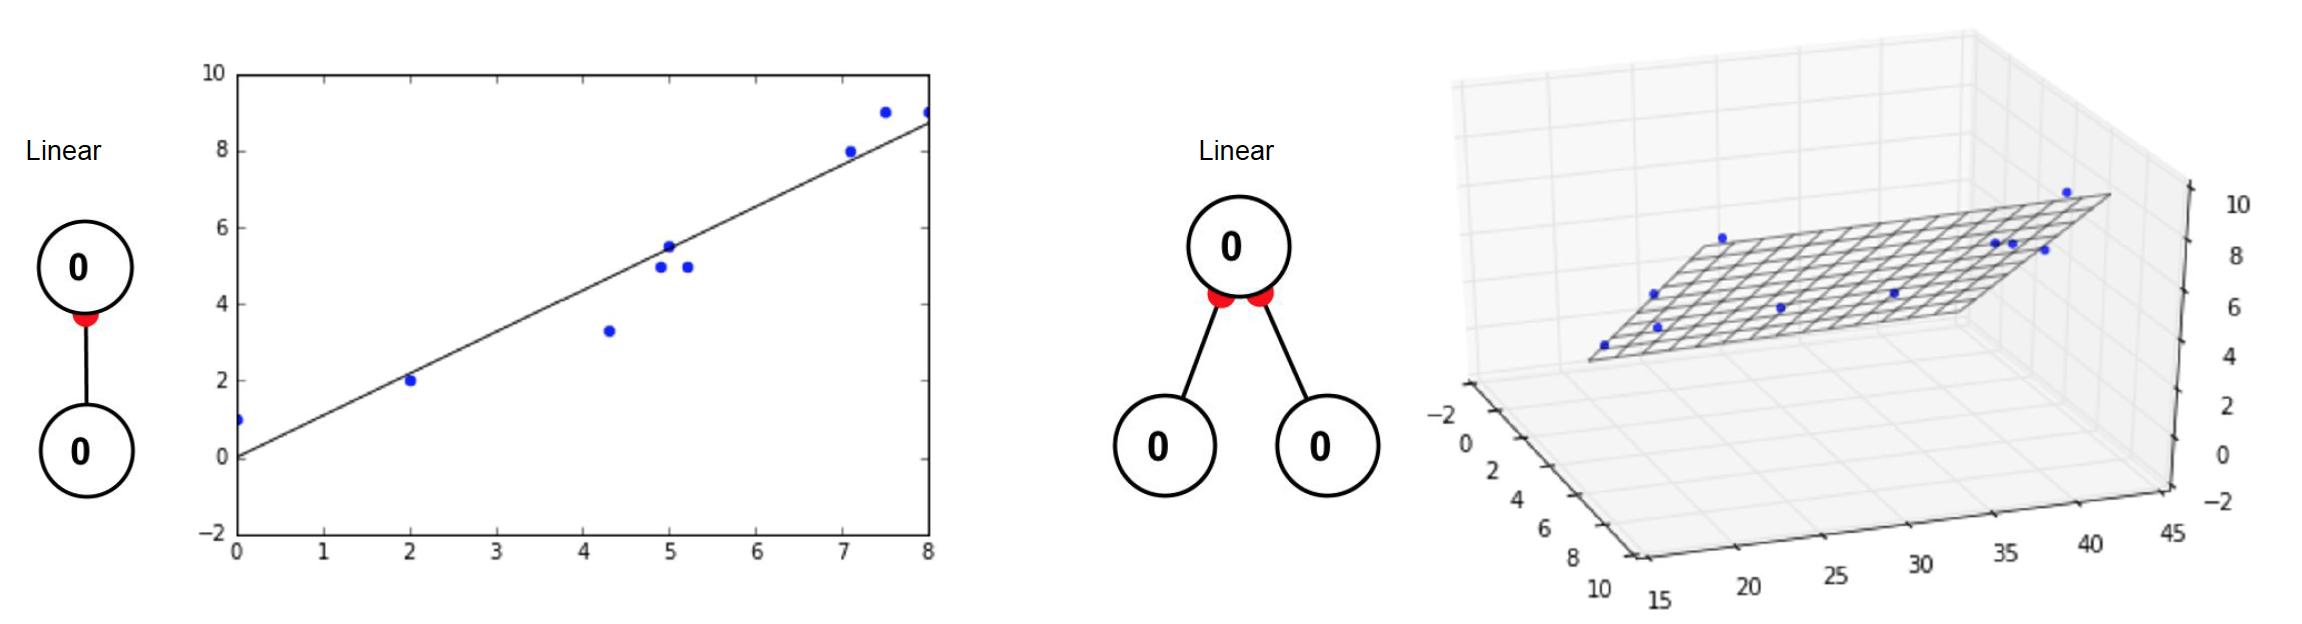
\includegraphics[scale=.4]{./images/visualizeRegression.png}
\caption[Jeff Yoshimi.]{A regression task for a 1-1 (Left) and a 2-1 network (Right) network of linear nodes. Datapoints in the input-target space are shown in  blue. The network implements a linear function from inputs to outputs, which is a line in the two dimensional input-target space on the left, and a plane in the three dimensional input-target space on the right. }
\label{visualize_regression}
\end{figure}
%In the regression case shown on the left, the output node has a linear activation function. We try to set the weight and bias of the network to fit the data. This is a \emph{graph of a function} and the space in the picture is the input-target space of that graph. 

Let's see how this works in a slightly larger network, a network with 2 input nodes and 1 output node, as in figure \ref{visualize_regression}, right. Here the graph of the function computed by the network is a 2-dimensional surface, and the input-target space of the graph is 3 dimensional (2 input nodes and 1 output node). Visualize the algorithm fitting that surface so that it's as close to the datapoints as possible. It's like fitting the line in the 1-1 network case, but now we have more knobs (the two weights and the bias of the output node) for moving the surface around. Each of the vectors in the 2-d input space is associated with a target value in the 1-d output space. The surface has been fit to the points, so that any input will be associated with outputs as close as possible to the target values. 

% The graph of function material could be more clear.
So here we have:
\begin{description}
\item[Regression hypersurface:] a generalization of the concept of a regression line to arbitrarily many dimensions. Mathematically it is the graph of an $n$-dimensional hypersurface, where $n$ is the number of input nodes. In the cases shown in figure \ref{visualize_regression} the hypersurfaces have 1 dimension (a line, for a neural network with 1 input node) and 2 dimensions (a plane, for a neural network with 2 input nodes). It is, in a sense, the ``solution'' a network learns for a regression problem. 
\item[Input-target space:] the space that the regression hypersurface lives in, which has as many dimensions as there are input nodes plus output nodes. The rows of the labeled dataset can be conceptualized as a cloud of datapoints in this space. The goal of regression is to make the hypersurface as close to that cloud of datapoints as possible. In the cases shown in figure \ref{visualize_regression} the input-target spaces have 2 dimensions (a neural network with 1 input node and 1 target node) and 3 dimensions (a neural network with 2 input nodes and 1 target node).
\end{description}

Notice that the decision boundary in figure \ref{visualize_classification} (right) looks like the regression line in figure \ref{visualize_regression} (left). Do not confuse these! In one case we have a decision boundary for a classification task computed by a 2-1 network; in the other case we have a regression line computed by a 1-1 network.

As soon as we have networks with more than 3 nodes, our ability to visualize things starts to break down. But we have experience thinking about shapes in higher dimensions (for example via our studies of dynamics in 4-dimensional state spaces, and recall our discussion of dimensionality reduction in section \extref{S:dimred}), so we should be able to do it. The regression hypersurface computed by a network has as many dimensions as there are input nodes. For example, if a linear network had 20 input nodes and 5 output nodes, its graph would be a 20-dimensional hyperplane fit to a cloud of points in a 25 dimensional space.

% Connect to generalization
% Mention universal approximations here?

\section{Error}\label{sect_error}

To assess how well a supervised learning algorithm is training a network to approximate a vector valued function, we  define an \glossary{error function}\footnote{These are also known as ``cost functions'', ``loss functions'', or ``objective functions''.} and then modify the weights and other parameters of a neural network to get the value of this error function to be as small as possible (compare the intuitive overview in Section \ref{SupervisedFirstPass}). An error function can be thought of as a method for producing a number which describes how well a network is doing at approximating the pattern-associations encoded by a labeled dataset. We call this the \emph{overall error}, since it is associated with the entire labeled dataset (as contrasted with errors associated with particular outputs). In learning, the goal is to use mathematical techniques to change the parameters of the network so that overall error is as small as possible.

% Check for \textbf above,  Also make sure all the _r's are outside of them!
In practice, to compute overall error, we compute errors for each row of the training subset of our labeled dataset. We go through each in vector $\mathbf{x}_r$ and see what output vector $\mathbf{y}_r$ the network produces. The resulting output dataset (see Chapter \extref{ch_data_science}) has the same number of rows and columns as the target dataset. We then go through each row $\mathbf{y}_r$ of the output dataset and compare it with the corresponding row $\mathbf{t}_r$ of the target dataset. We often end up comparing things like $\mathbf{t}  =  (1,1)$ and $\mathbf{y}  =  (.9,.7)$ by subtracting the components of the two vectors, which gives us  errors $(1-.9,1-.7) = (.01,.03)$.\footnote{At the level of an individual node, an error is just the difference between what we wanted and what we get, a target value minus an output value.}

% Error is the flip side of \glossary{performance}. Reducing the error in a network improves its performance. We want to maximize performance by minimizing error.\footnote{In fact any optimization problem can either be thought of in terms of minimizing a cost function or, equivalently, as maximizing the negative of the cost function, which we are calling performance.}  Deep learning discussion of error vs. performance where they are not just symmetrical opposites. Around 268, section 8.1

The concept of error should be intuitive. If we want our network to produce the output vector $(1,1,1)$ but instead it produces $(-1,0,.2)$, we have a few errors in the output. But if we train it and it starts to produce the output vector $(1,1,.9)$, then we are doing much better! The first output is about 4 units ``off'', but the second output is about $.01$ off. That's all the basic idea involves. Saying this mathematically requires some notation, but remember all we're ultimately doing is finding a number that says how far ``off'' the outputs are from the target values.

% Add reference here once there is more discussion in the book, in particular of cross entropy
There are many error functions that we can use to compute overall error.\footnote{One main consideration is whether you are training a network on a classification task or a regression task.  A common error function used in classification tasks is cross-entropy.  Sum squared error, which we consider here (or its close cousin mean squared error), is usually used for regression tasks, but it can also be used for classification, so it's a good example to start with.} Here we are just introducing the basic idea. We focus on an error function called \emph{sum of squared error} or SSE.\footnote{This presentation of SSE combines two separate sums: a sum over the components of a single error vector for one row of training data, and a sum over all of these individual ``row errors'' in a training set or batch. However, ``SSE'' is often reserved for the first sum, which is for one row only.  Then in a separate step we reduce all of the row errors in a batch to an overall error, either by taking a sum or mean of row errors. So we can have overall error as the mean or sum of the SSE for each row, or as the sum or mean of MSE for each row. These distinctions cannot be made using the current presentation, and so we plan to disaggregate these concepts in a future version of this chapter.}  

Suppose we are given a network and labeled dataset, and have computed the output dataset. To compute SSE, we go through each row and subtract each output value from the corresponding target value. This gives an error value for each row. We then square these errors and add the squared errors together. That is the sum of squared errors. Figure \ref{error_computation1} shows the computation for the case where there is a single output node.\footnote{In these figures, $\sum_R$ is shorthand for $\sum_{r=1}^{R}$.}  In the case shown, outputs are very close to targets, and so the SSE is pretty low:

\begin{figure}[h]
\centering
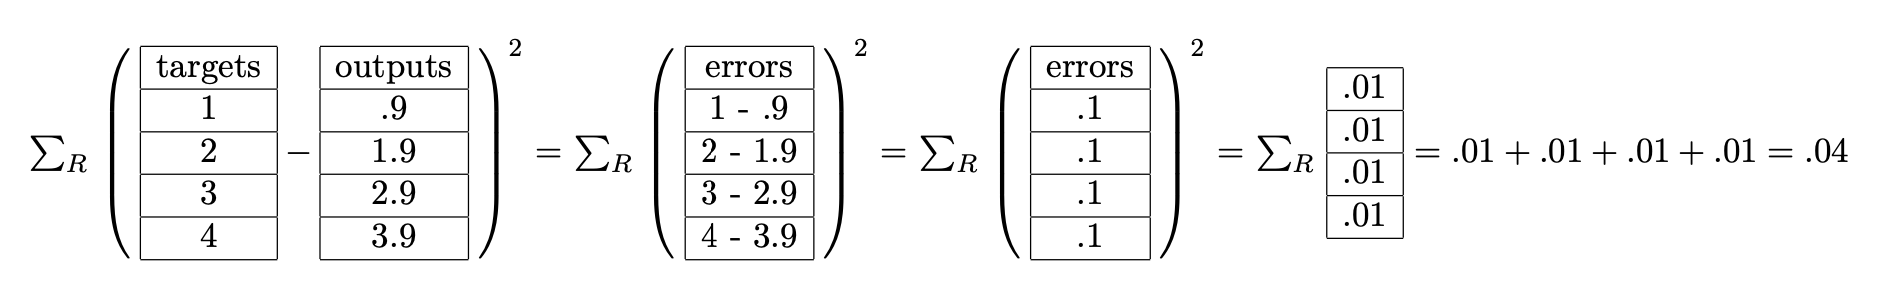
\includegraphics[scale=.5]{./images/ErrorComputation_1.png}
\caption[Jeff Yoshimi.]{Computing SSE for a network with one output node. As can be seen, each output is just $.1$ below the target, and so SSE is pretty low. }
\label{error_computation1}
\end{figure}

% TODO: Often this is written using double brackets, as in ||t - y||^2. Given the convention, maybe favor something more like that
The same idea works  for a network with more than one output node, but in that case the squaring operation must be defined for vectors. All this really amounts to is squaring target - output for each output value, and then adding the results together, and it turns out we can express this concisely using some of the vector operations we learned in the linear algebra chapter (chapter \extref{ch_linear_algebra}): 
% Spelled out version of the error, but not sure it helps, and this notation would have to be worked out
%\begin{eqnarray*}
%SSE =  \sum_{r=1}^{R}  \sum_{i=1}^{N} (t_{r_i} - o_{r_i})^2
%\end{eqnarray*}
\begin{eqnarray*}
SSE =  \sum_{r=1}^{R}(\mathbf{t}_r - \mathbf{y}_r) \bullet (\mathbf{t}_r - \mathbf{y}_r) 
\end{eqnarray*}
That is, for each row $r$, we subtract the output vector from the target vector using component-wise subtraction, and then take the dot product of the resulting vector with itself to get the squared error for that row. For example if $\mathbf{t}_1 = (1,1)$ and $\mathbf{y}_1 = (2,3)$, then  $(\mathbf{t}_1 - \mathbf{y}_1) = (1,1) - (2,3) = (1-2,1-3) = (-1,-2)$. We ``square'' this vector of errors by dotting it with itself: $(-1,-2) \bullet (-1,-2) = -1^2 + -2^2 = 5$. 

Sample computations for a network with two outputs are shown in figures \ref{error_computation2_low} and \ref{error_computation2_high}.  Notice that SSE is low in figure \ref{error_computation2_low}, and higher in figure \ref{error_computation2_high}. 

\begin{figure}[h]
\centering
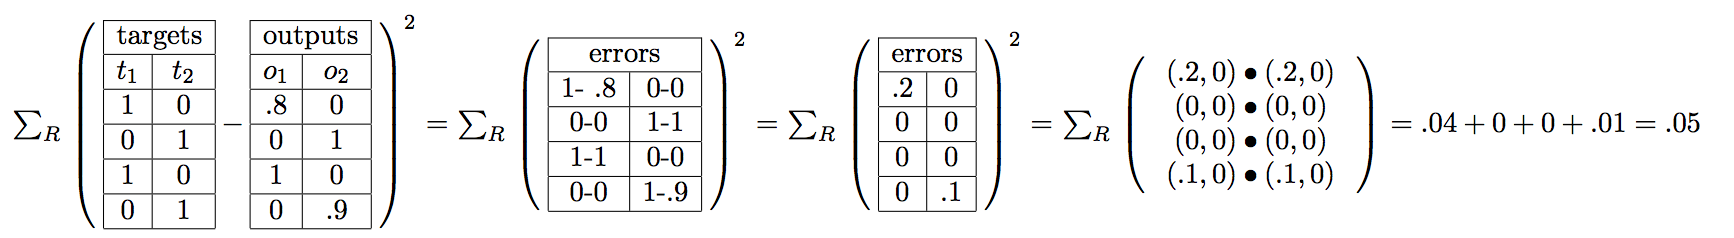
\includegraphics[scale=.5]{./images/ErrorComputation_2_low.png}
\caption[Jeff Yoshimi.]{Computing SSE for a network with two outputs. Error is fairly low.}
\label{error_computation2_low}
\end{figure}

\begin{figure}[h]
\centering
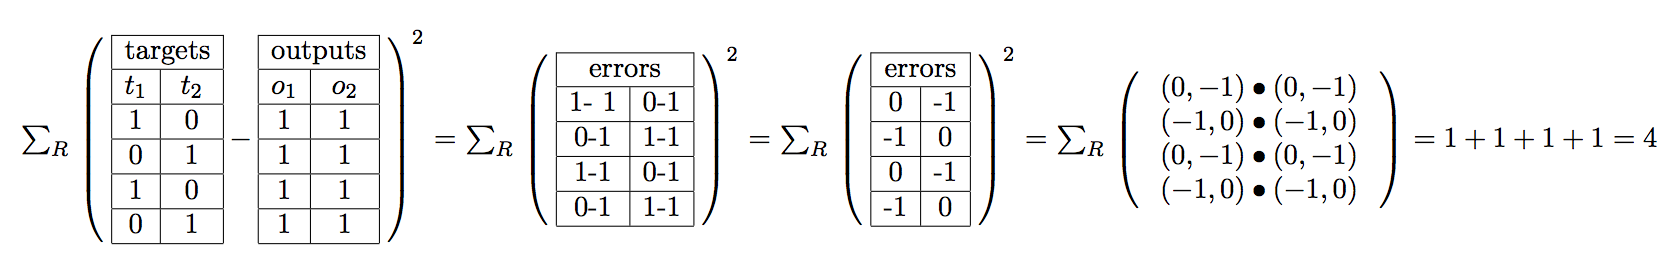
\includegraphics[scale=.5]{./images/ErrorComputation_2_high.png}
\caption[Jeff Yoshimi.]{Computing SSE for a network with two outputs when error is higher, as might happen when we start with random weights, which, for example, cause the outputs to always be 1.}
\label{error_computation2_high}
\end{figure}

Low overall error (here low SSE) is something we generally see \emph{after} training a  network. When we start with an untrained network that has random weights, error will be higher, as in figure \ref{error_computation2_high}.

Try some examples of your own to get a feel for when SSE is large vs. small.

Learning algorithms minimize SSE and other overall error metrics relative to training subset of the labeled dataset. However, it is usually important to hold out some testing data as well, to see how well the network generalizes to data it was not trained on. Thus we often have two measures of error when we are done training a network: error for the training data, and error for the test data (see section \extref{generalization}).

\section{Error Surfaces and Gradient Descent}\label{sect_gradient_descent}

Before we get to the main point of this section--gradient descent--we need to do a bit more visualizing. We are going to talk about \emph{another} type of graph, separate from the ones discussed in sections \ref{visClassification} and \ref{visRegression}. We will be talking about parameter spaces, or to make things easier, weight spaces (recall these have come up in chapters \extref{ch_dst} and \extref{ch_unsupervised}). On top of the weight space we will plot overall errors. That is, for each possible combination of weight values, we show what overall error (\eg SSE) would result relative to our network and training set. This  gives us an \glossary{error surface}. 

Note that error surfaces depend on the training set, and in particular targets, because this determines SSE. If you change the training set, you change the error surface. Once you fix the training set, you can now look at the error surface, which shows all possible errors for that network \emph{given} the training set.
% it can also change we change how we compute error or cost / loss more generally. 

Figure \ref{error_surfaces} shows errors surfaces for two cases that we can visualize. On the left we have an error surface for a 1-1 network where we are only adjusting a single weight. As we change that weight, SSE will change too. On the right we have a 2-1 network where we are adjusting two weights. Again, as the two weights are changed so will the SSE. Notice that in each case the error surface has a single minimum point, which turns out to be convenient: our goal, after all, will be to find that lowest point, the configuration of weights where overall error is lowest.  But we are not always lucky enough to get such a surface, as we will see.
% Convexity, when this is the case

\begin{figure}[h]
\centering
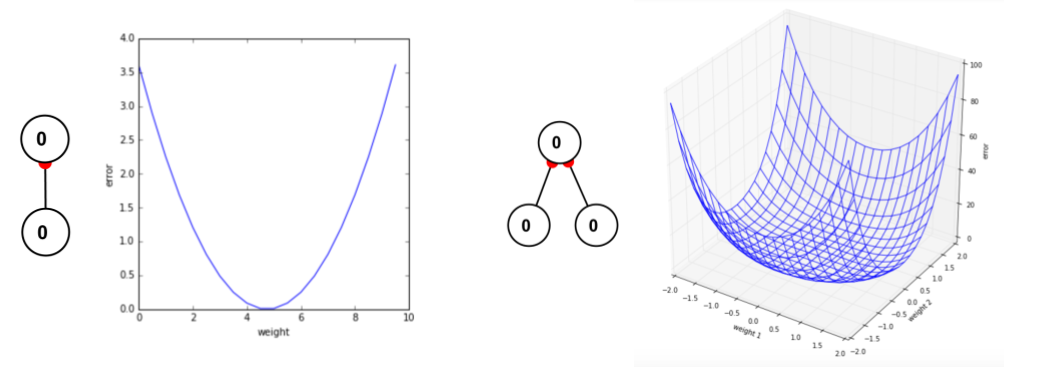
\includegraphics[scale=.5]{./images/ErrorSurfaces.png}
\caption[Jeff Yoshimi.]{(Left) error surface for a 1-to-1 network where only the weight is adjusted. (Right) Error surface for a 2-to-1 network where the two weights are adjusted. In each case, the error surface also depends also the training data (the tables in figure \ref{tables_nets}). }
\label{error_surfaces}
\end{figure}

% Make connection to graph of function?
These ideas generalize to higher dimensions, for networks with many parameters. As above, we can't visualize these cases directly, but it helps to have a visual template in mind. The error surface for a network with $n$ adjustable parameters is a surface in an $n+1$ dimensional space (the $n$ parameters plus the error term). For a network where we are adjusting three weights, we have the graph of a function from the three weights to the error, \ie a surface in a 4-dimensional space. For each possible combination of three weights, we can generate an error, and thus we have an error surface in a 4-d space. For a network with 150 weights, we have an error surface in a 151 dimensional space.

For supervised learning tasks (regression or classification), our goal is usually going to be to \emph{minimize the overall error function}. We want to find values for the parameters that make overall error, relative to the labeled dataset, as low as possible. It turns out there is a whole area of mathematics set up for problems like that. It's called \glossary{optimization}.\footnote{\url{https://en.wikipedia.org/wiki/Mathematical_optimization}.} Optimization problems involve finding either the minimum value or maximum value of a function, relative to the set of all possible inputs to the function. Here the function is the error function and the inputs are adjustable parameters, usually weight strengths and node biases. 

Optimization is useful. We often have to make decisions that involves many different variables and constraints. For example, suppose you want to buy a new laptop. You want the cost to be as low as possible, but the quality as high as possible. You need to buy it within 5 days and you really want a warranty. Often what you do is look at choices. When a tentative choice feels  better, you go in that direction. If it feels worse  you might tell yourself  ``no, I dislike that, look for something else''. In this way you go back and forth--generally in the direction of ``better''--and settle in on a solution. Once again, the Goldilocks principle. 

Optimization automates this kind of process, providing an automatic way to solve this kind of problem. Optimization methods are used, for example, to determine the best ways to plant crops to maximize yield. Supervised learning methods also make use of optimization. A labeled dataset describes an optimization problem, a set of inputs that we want to associate with a set of targets. Mathematical optimization gives us a way to automatically update the parameters of a network so that it does the best job possible on a classification or regression task, producing outputs in response to inputs that are close as possible to their targets.
% Above add reference to generalization. We also want networks that generalize well.

\begin{figure}[h]
\centering
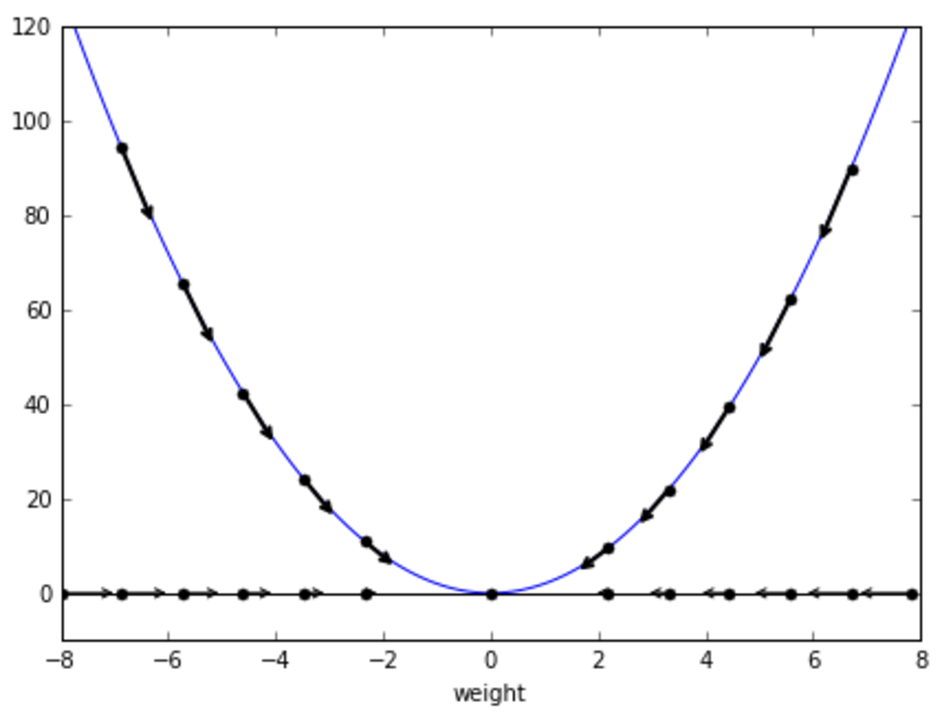
\includegraphics[scale=.5]{./images/GradientDescent.png}
\caption[Jeff Yoshimi.]{Error gradient on an error surface. The actual changes that happen in the weight space are shown on the horizontal axis.}
\label{gradient_descent}
\end{figure}
% Note this is not what we tend to see. In practice, different shapes. And some have tried to visualize these structures.

The main method we will discuss for minimizing the error function is  \glossary{gradient descent}.\footnote{The gradient of an error function is a vector that points in the direction of steepest increase on the error surface. The method of gradient descent involves changing a system in the direction of steepest decrease on the error surface, which is the negative of the gradient of the error function.}  In this method we start at some random point in parameter space. We begin with a network where the weights and biases and other adjustable parameters are set to random values. In the 1-to-1 network we just randomize that one weight. That puts it at a random place on the error surface over the weight space in figure \ref{error_surfaces} (left). Using the tools of calculus, we can then attach an arrow to any point on the error surface, which says in what direction the surface is decreasing most rapidly.\footnote{An excellent discussion of the calculus relevant to neural networks is \url{https://explained.ai/matrix-calculus/.}} So we start at a random point, follow the arrow down from there (changing the weights to new values), and then repeat the process. By iterating the algorithm in this way we ``descend the gradient.''

The process is illustrated in figure \ref{gradient_descent}. The error surface has a bowl shape. Wherever you start in the bowl, just follow the arrows down until you get to the low point. That's it!  That's how it works. 
% Convex guaranteed to have no more than one minimum, thought it might have none. You will have none or one.

We use the ``arrows'' on the error surface to derive a learning rule, which produces a \emph{dynamical system on weight space}. In chapter \extref{ch_dst} we mainly considered activation dynamics. Here we consider weight dynamics. The weight dynamics are shown in the bottom horizontal line of the figure; in that line a one-dimensional system describing how a single weight changes in order to implement a model of the training data. As noted in chapter \extref{ch_dst}, when a ``play''  button 
\includegraphics[scale=.5]{./images/Play.png} is pressed in Simbrain  a dynamical process is simulated. In this case we will have a tools in Simbrain for running gradient descent using a play button, and observing error reduction.\footnote{See the screenshot here: \url{http://www.simbrain.net/Documentation/v3/Pages/Network/training/trainingDialog.html}.} What we are doing is like what we did there when we looked for fixed points of a recurrent network. Here the initial conditions are random weight values, which put us at a random point in the error surface, orbits are the paths we follow in weight space (which is our state space in this case), and we usually end up  at an attracting fixed point, a weight state with low error. 

% Mention convexity below?
% Possibly clarify that global minimum is itself a local minimum (local connotes neighborhood of state space)
Unfortunately, error surfaces don't always have just a single minimum point, as in the bowl example (if they did, training networks would always be easy). They sometimes have multiple fixed points in separate basins of attraction. These are ``local minima''. Error surfaces can also have plateaus where the error will only gradually change. Both cases are shown in figure \ref{local_minima}. These can make finding the best solution difficult. Much of the mathematical theory of optimization (and  research in neural networks) is focused on dealing with these ``difficult'' error surfaces.

We usually don't have a picture of an error surface. Still, we can use a program like Simbrain to get a feel for an error surface. To do so, we start at a random point in weight space, run the algorithm, and then see what the lowest error we get is. If it does not seem so low, we try again.\footnote{It's easy to try this in Simbrain. Load up a backprop network with a training set, and train. Periodically press the random button and run again, and notice how the error changes each time. Again, this is almost exactly the same as searching for fixed points of a dynamical system,  with the state space here being a weight space.} By repeatedly doing this we get a feel for how many minima they are and how long it takes to get to them. Of course, for very  large networks, where training can take hours or days, we can't to this, but for small toy networks we can.

\begin{figure}[h]
\centering
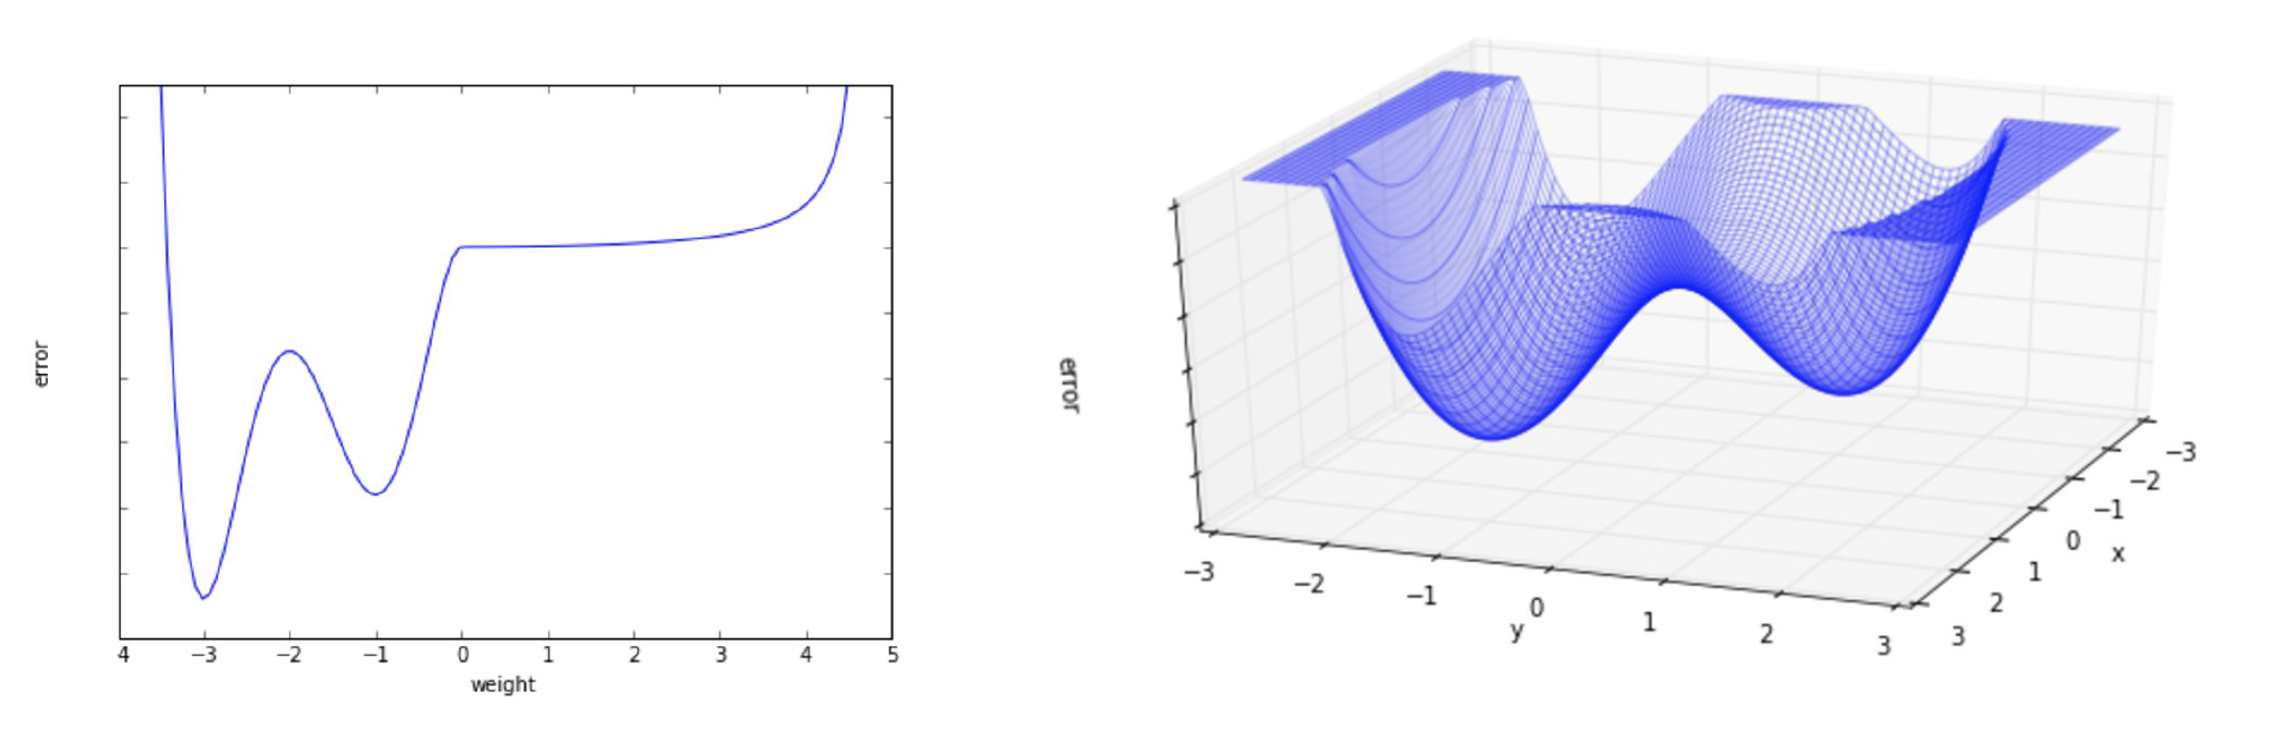
\includegraphics[scale=.4]{./images/LocalMinima1d2d.png}
\caption[Jeff Yoshimi and Scott Hotton.]{(Left) an error surface for one weight, with two local minima and a plateau. (Right) An error surface for two weights, with two local minima.}
\label{local_minima}
\end{figure}
% Label the global, local minima and plateaus

 There is more to say here. A lot can go wrong, there are settings to adjust (like \emph{how far} you go at each iteration), etc. These details are studied in the mathematical field of optimization. 
 % Point to another source, preferably open access
 
 \section{Expansion of these methods}
 
 This chapter has described some very general features of supervised learning. The history and details of how these are applied in particular cases is spelled out in subsequent chapters.  In chapter \extref{ch_lms_backprop} we see details of this type of algorithm for the case of a simple one-weight-layer network, and then we see how backprop allowed the algorithm to be generalized to feedforward networks with more than weight layer. The key was calculus: by figuring out how to update parameters to reduce error using calculus, a systematic method for applying gradient descent to more complex networks was found.
 
 % glossary items for automatic differentiation and computational graphs
One feature of the revolution in neural networks that began around 2010 (see section \extref{deep_revolution}) is that these techniques became in a certain sense automated. Libraries were introduced that made it possible to define any kind of layer and link between layers, and as long as certain structures were defined, the calculus could be done automatically, allowing gradient descent to be used.  This is sometimes called automatic differentiation, and it can be done on an arbitrary computational graph.  That made it possible to really define all kinds of crazy networks and structures and layers and update rules and train them using tradient descent. Examples include convolutional layers (chapter \extref{ch_cnn}) and transformers  (chapter \extref{ch_transformers}).
 
Because these methods are so powerful, it's often useful to find ways to apply them even when it seems they don't apply. For example, as we see in chapters \extref{ch_supervised_recurrent} and \extref{ch_reservoir}, there are various ways it has been possible to use these same techniques--which work best with feedforward networks--on or with recurrent networks.  
 
\section{SSE Exercises}

\newcounter{SSECounter}

\noindent
\stepcounter{SSECounter}
{\bf \theSSECounter.}  Given targets $(0,1,0)$ and output activations $(1,1,1)$ what is SSE? \\
{\bf Answer:}  \\
$(0-1)^2 + (1-1)^2 + (0-1)^2 = 1 + 0 + 1 = 2$
\bigskip

\noindent
\stepcounter{SSECounter}
{\bf \theSSECounter.}  Given targets $(1,1,1)$ and output activations $(2,-1,-2)$ what is SSE? \\
{\bf Answer:}  \\
$(1-2)^2 + (1- (-1))^2 + (1-(-2))^2 = 1 + 4 + 9 = 14$
\bigskip

\noindent
\stepcounter{SSECounter}
{\bf \theSSECounter.}  Given targets $(1,1,1)$ and output activations $(1,1,1)$ what is SSE? \\
{\bf Answer:}  \\
$(1-1)^2 + (1-1)^2 + (1-1)^2 = 0 + 0 + 0 = 0$
\bigskip
